{
\usebackgroundtemplate{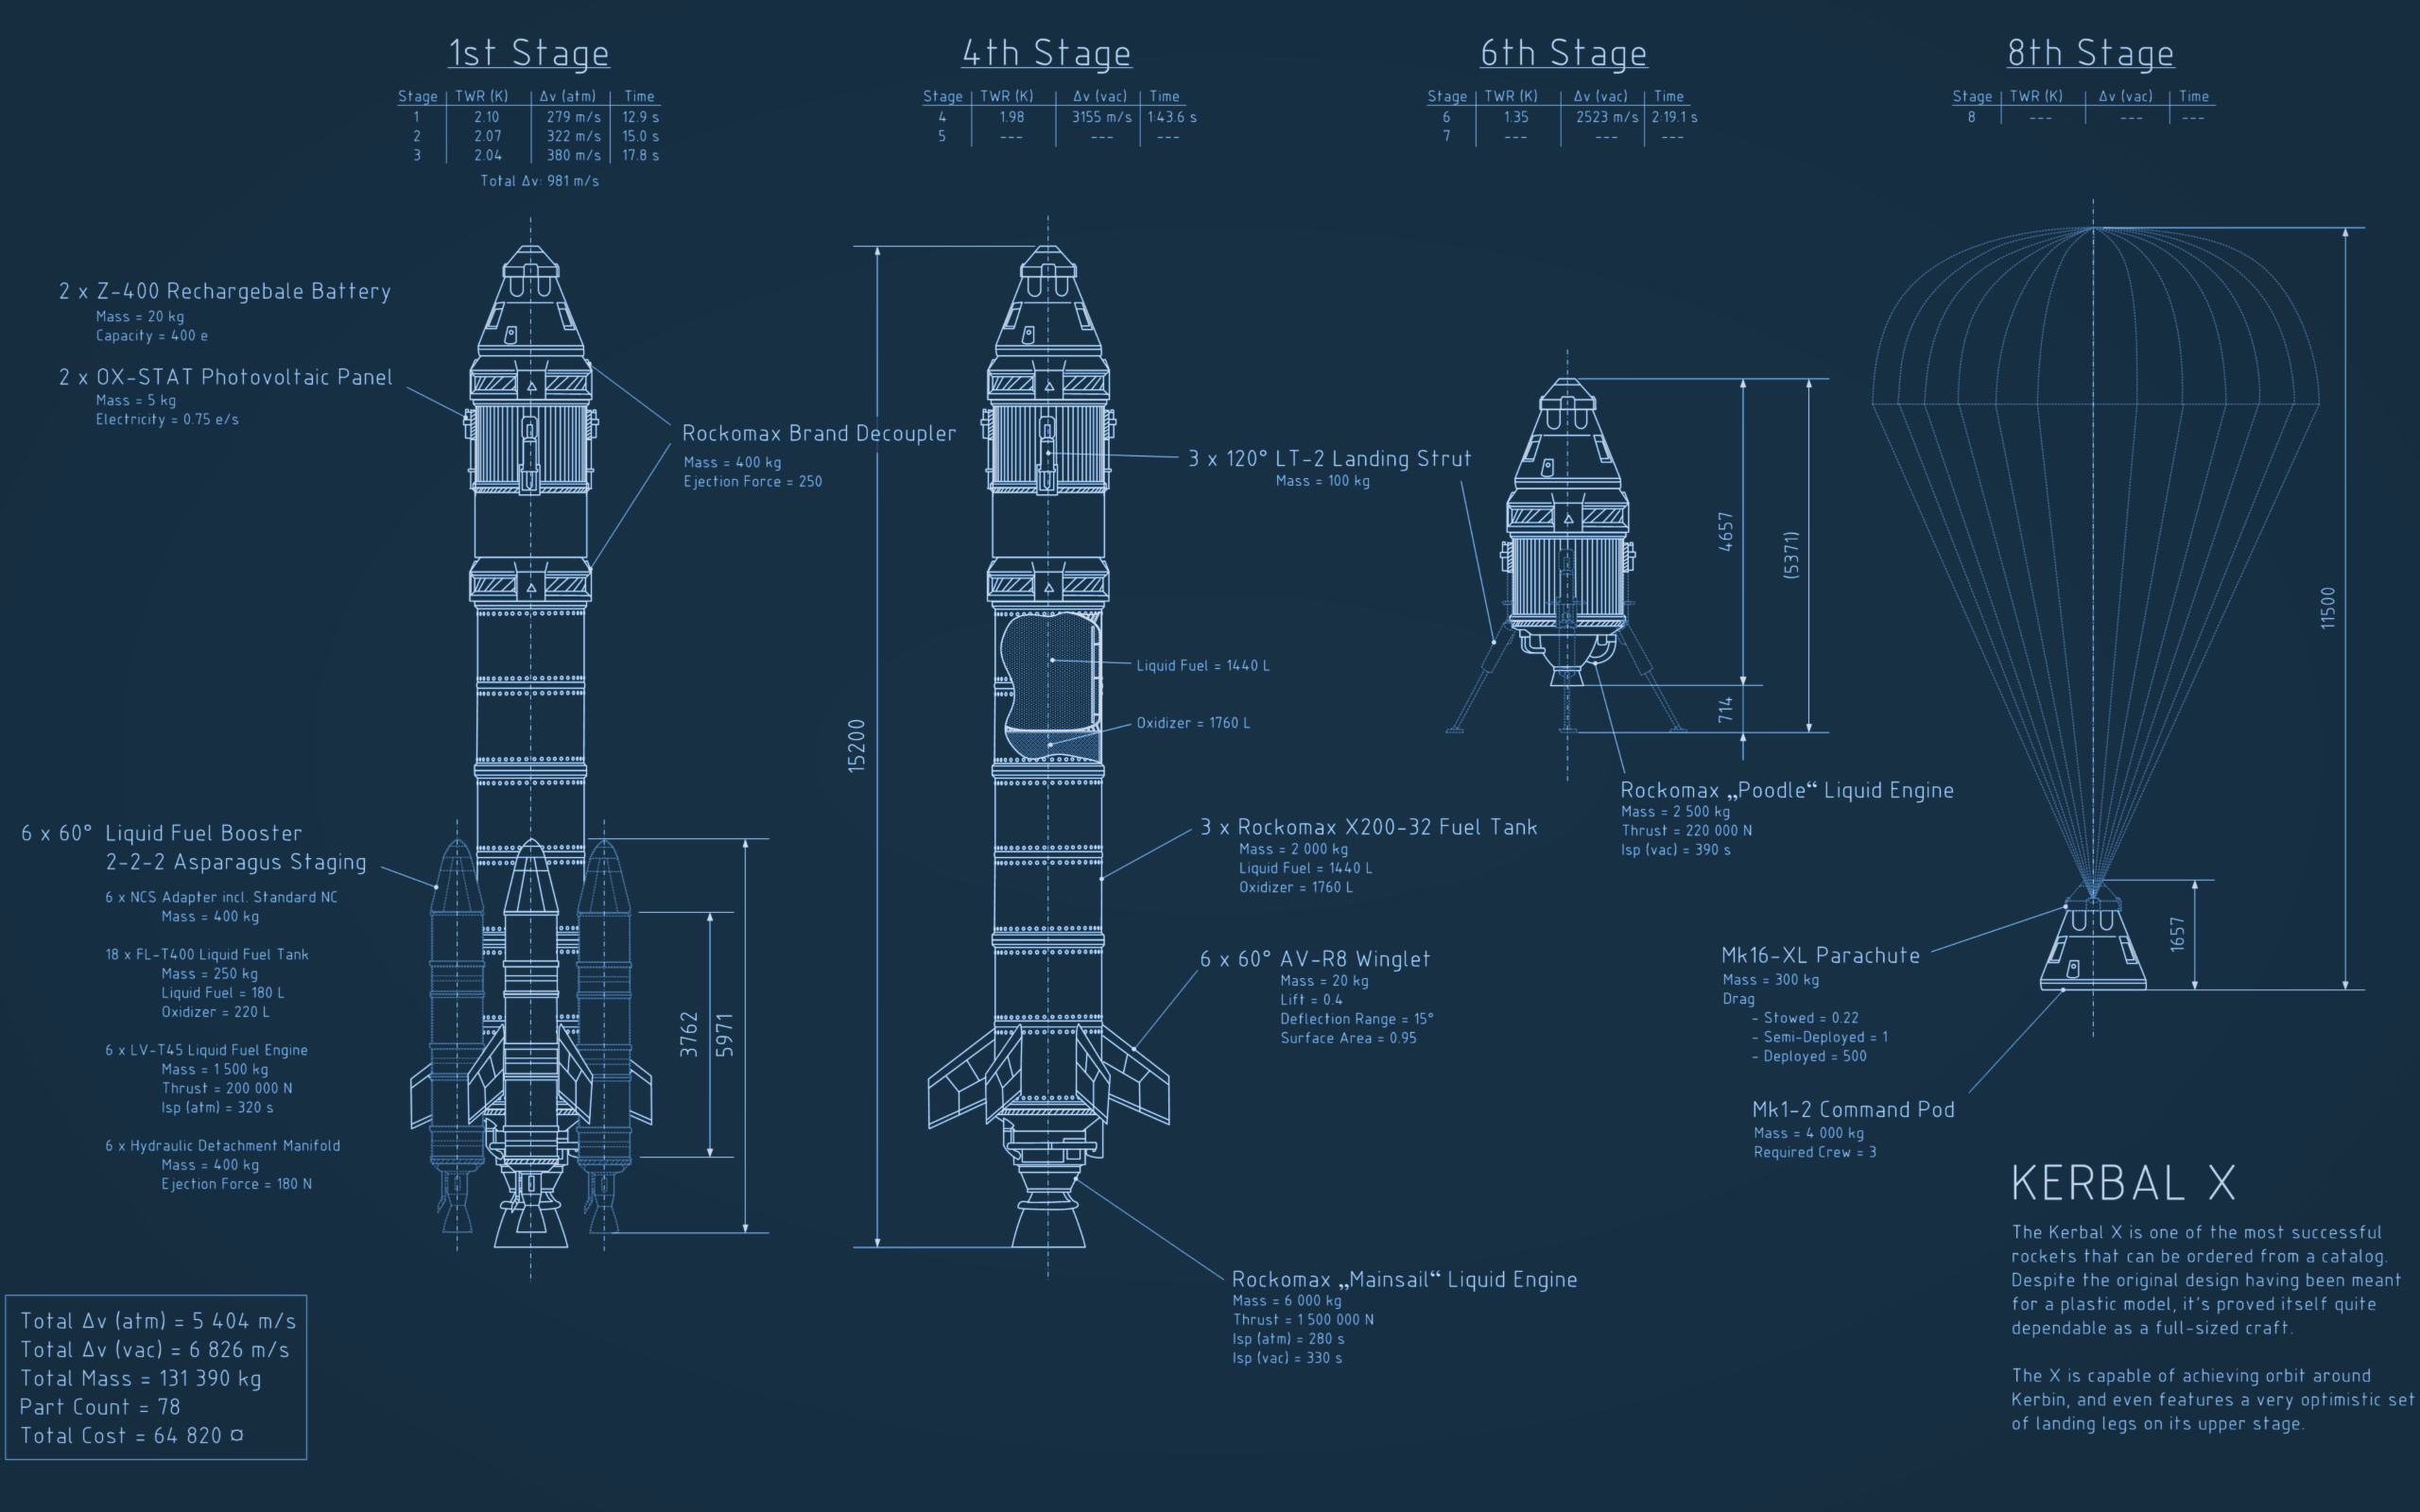
\includegraphics[width=\paperwidth]{images/staging.jpg}}%
\begin{frame}
\end{frame}
\begin{frame}
    \frametitle{Staging}
    \begin{block}{How do we do it}
        \begin{itemize}
            \item Split the rocket in 2 or more parts.
            \item Each part carries own fuel and engine
            \item Each part can be seperated from the rocket in sequence
            \item e.g. booster stage, landing stage, transfer stage, ...
        \end{itemize}
    \end{block}
\end{frame}
\begin{frame}
    \frametitle{Staging}
    \begin{block}{Why do we do it}
        \begin{itemize}
            \item Rocket efficiency is inversly proportional to it's weight
            \item Delta-v goes up as total mass decreases
            \item We want to carry as little mass as posible
            \item Throw away excess weight of unused engines and empty fueltanks
        \end{itemize}
    \end{block}
\end{frame}
}
\begin{frame}
    \frametitle{Staging}
    \begin{block}{}
        \begin{center}
            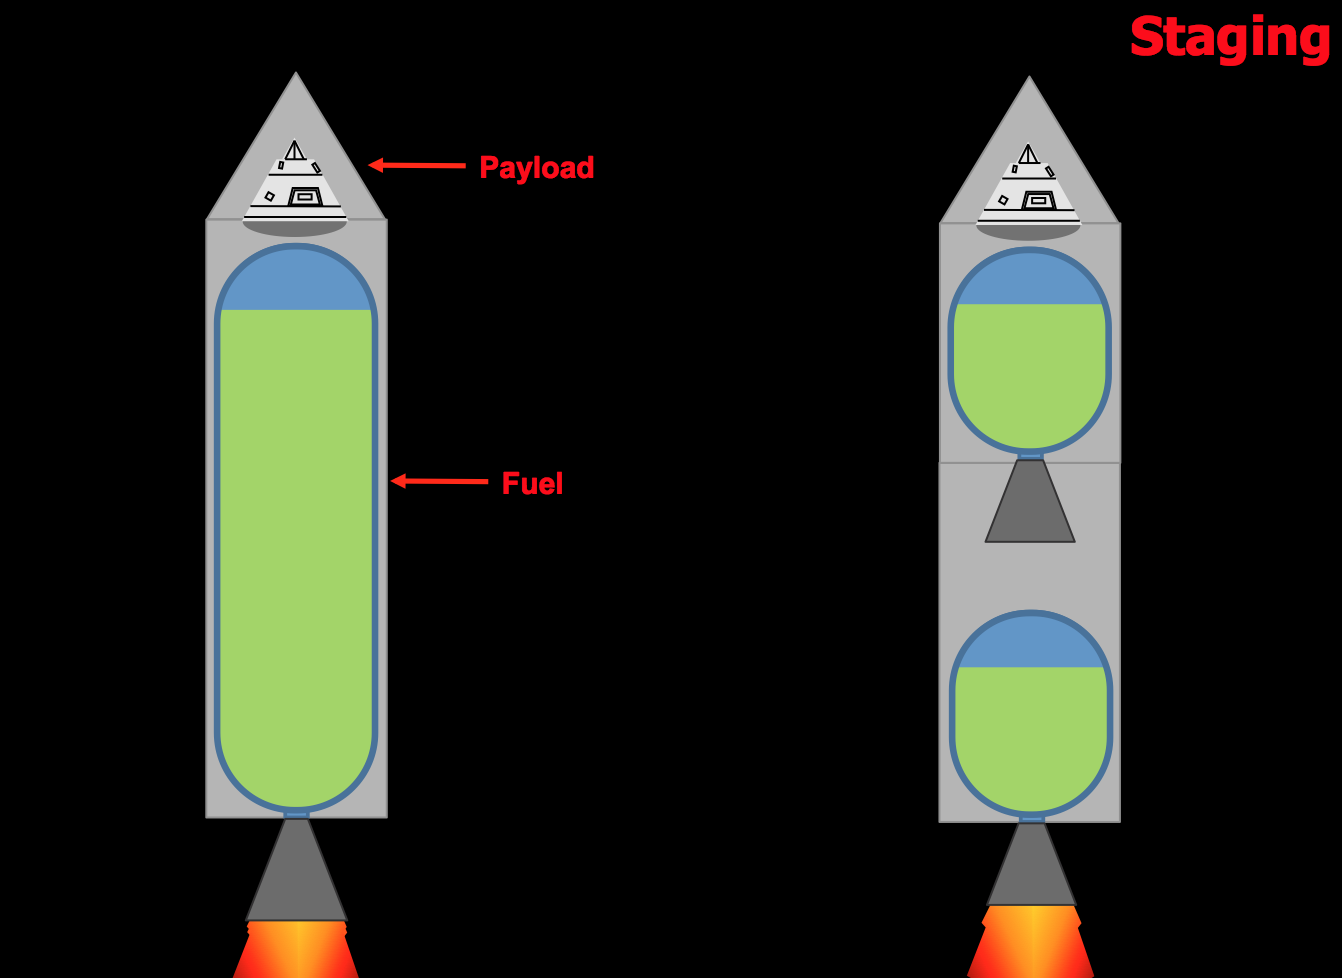
\includegraphics[width=0.5\textwidth]{images/staging1.png}
        \end{center}
    \end{block}
\end{frame}
\begin{frame}
    \frametitle{Staging}
    \begin{block}{}
        \begin{center}
            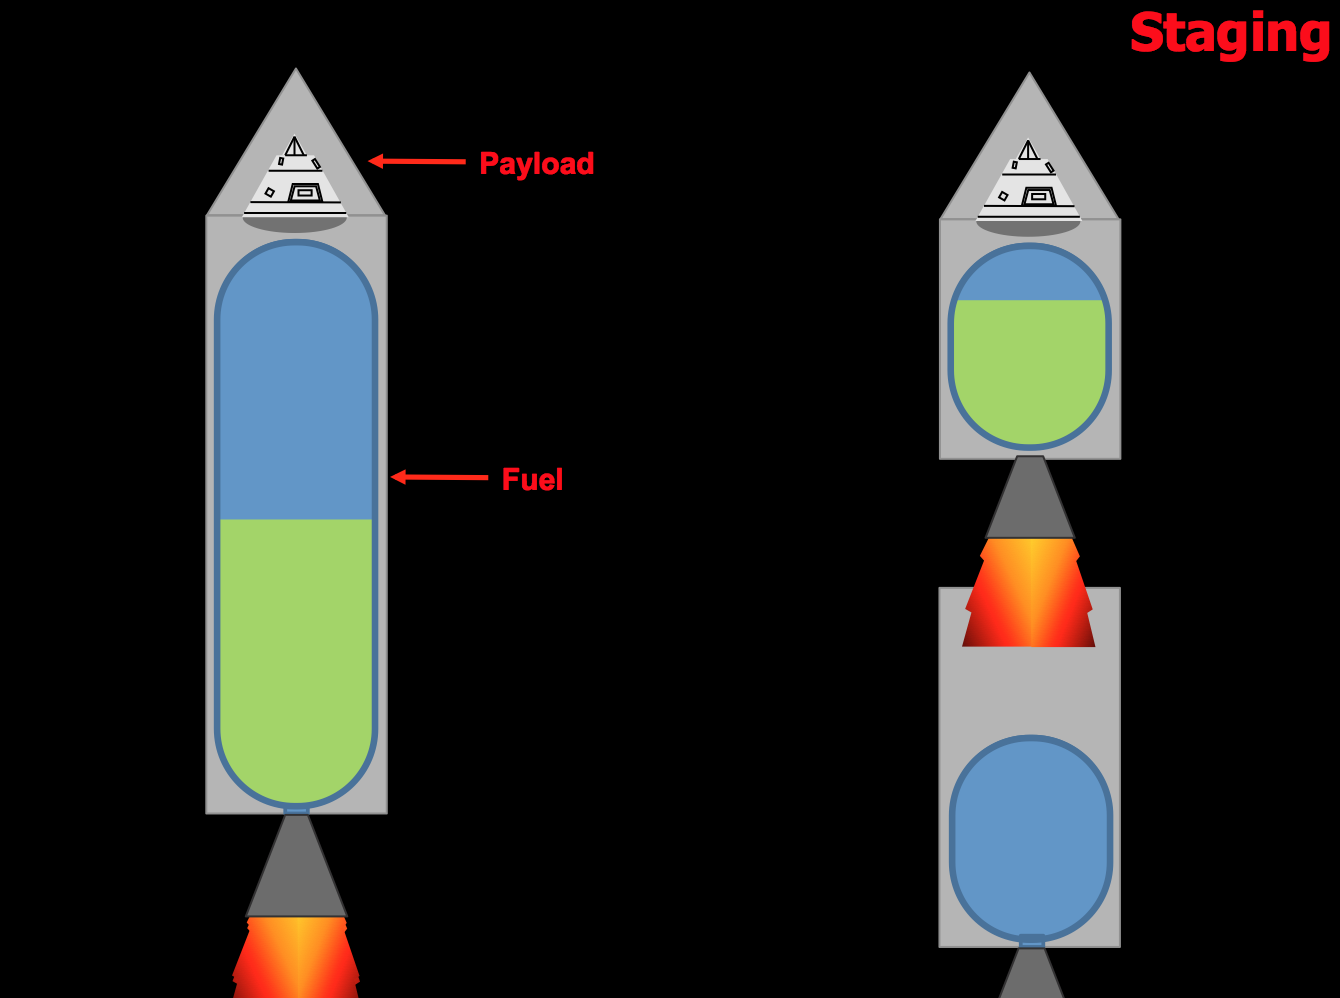
\includegraphics[width=0.5\textwidth]{images/staging2.png}
        \end{center}
    \end{block}
\end{frame}

{
\usebackgroundtemplate{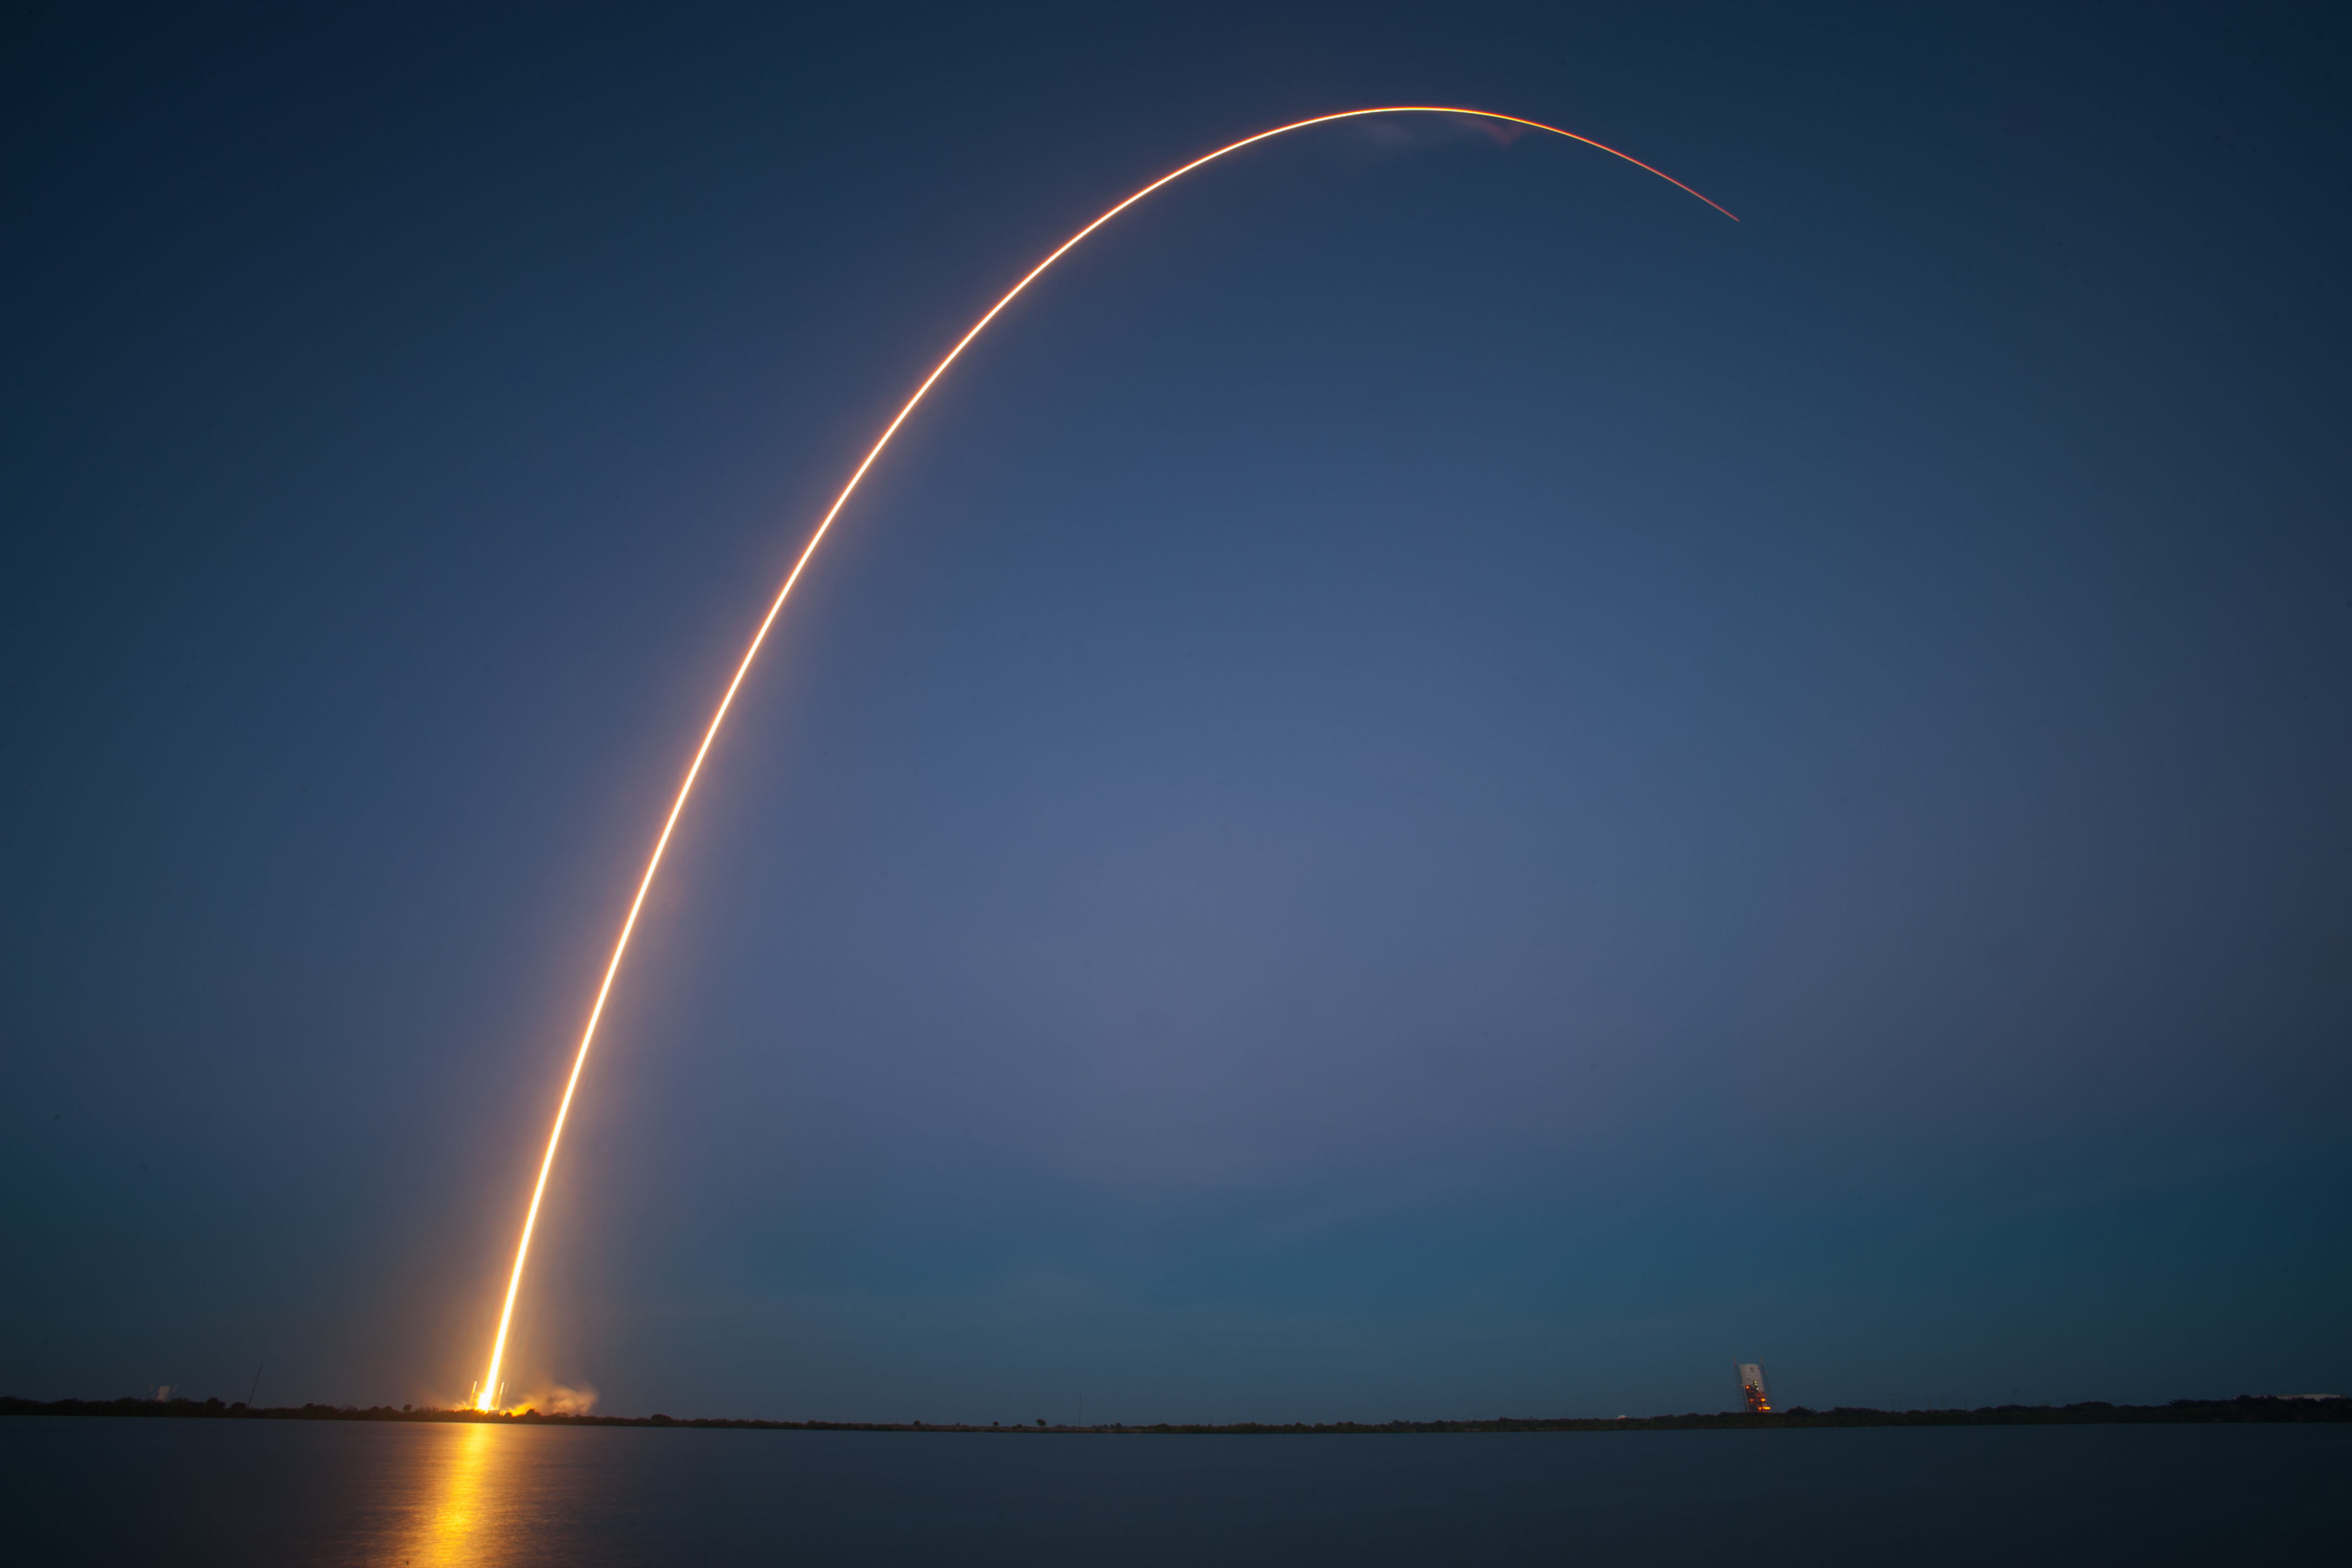
\includegraphics[width=\paperwidth]{images/gravity_turn.jpg}}%
\begin{frame}
\end{frame}
\begin{frame}
    \frametitle{Gravity turn}
    \begin{block}{Why do we turn}
        \begin{itemize}
            \item going straight up gains altitude more quickly
            \item but we would just fall down again
            \item we need to move sideways too in order to achieve orbit
        \end{itemize}
    \end{block}
\end{frame}
\begin{frame}
    \frametitle{Gravity turn}
    \begin{block}{Why to the east}
        \begin{itemize}
            \item Rotation of earth is already moving us towards the east at 1.5km/h
            \item escape velocity of earth is just over 7km/s
            \item rotational velocity is higher around the equator that why we want to launch from Cape Canaveral
            \item 1.5km/h does not seem to be a lot compared to 7km/s but keep in mind that we are heaviest at the start of launch.
        \end{itemize}
    \end{block}
\end{frame}
\begin{frame}
    \frametitle{Launch}
    \begin{block}{How do we do it}
        \begin{itemize}
            \item throttle up
            \item point at the right angle
            \item don't. touch. anything. let gravity do it's work
            \item activate staging at the appropriate times
            \item keep apoapsis in front of you untill desired hight
            \item circularize orbit
            \item It easy, it's not ro... oh...
        \end{itemize}
    \end{block}
\end{frame}
}
